\documentclass[11pt]{article}

\hoffset        2mm 
\voffset        -15mm
\oddsidemargin  0mm
\topmargin      0.5in
\textwidth      6in
\textheight     9in

\usepackage{graphicx,amsmath, amssymb, amsthm, amsfonts}


% Define the theorem styles and numbering
\theoremstyle{plain}
\newtheorem{theorem}{Theorem}[section] % changed counter "chapter" to "section" for use in an article
\newtheorem{proposition}[theorem]{Proposition}
\newtheorem{corollary}[theorem]{Corollary}
\newtheorem{lemma}[theorem]{Lemma}

\theoremstyle{definition}
\newtheorem{definition}[theorem]{Definition}
\newtheorem{example}[theorem]{Example}

\theoremstyle{remark}
\newtheorem*{remark}{Remark}
\newtheorem*{claim}{Claim}




%% Create shortcut commands for various fonts and common symbols
%\newcommand{\k}{\kappa}
\newcommand{\C}{\mathbb{C}}
\newcommand{\veps}{\varepsilon}
\newcommand{\eps}{\epsilon}
\newcommand{\f}{\textbf{f}}
\newcommand{\fb}{\textbf{f}}
\newcommand{\F}{\mathbb{F}}
\newcommand{\Fb}{\textbf{F}}
\newcommand{\gb}{\textbf{g}}
\newcommand{\h}{\textbf{h}}
\newcommand{\kb}{\textbf{k}}
\newcommand{\M}{\mathcal{M}}
\newcommand{\N}{\mathbb{N}}
\newcommand{\Norm}{\textbf{N}}
\newcommand{\n}{\textbf{n}}
\newcommand{\vp}{\varphi}
\newcommand{\vph}{\hat{\varphi}}
\newcommand{\p}{\phi}
% note:  \P is already defined to be the paragraph symbol
\newcommand{\Proj}{\mathbb{P}}
\newcommand{\Pcal}{\mathcal{P}}
\newcommand{\Q}{\mathbb{Q}}
\newcommand{\R}{\mathbb{R}}
\newcommand{\rb}{\textbf{r}}
\newcommand{\s}[1]{\mathcal{#1}}
\newcommand{\supp}{\text{supp}}
\newcommand{\Surf}{\textbf{S}}
\newcommand{\tpsi}{\tilde{\psi}}
\newcommand{\ub}{\textbf{u}}
\newcommand{\U}{\textbf{U}}
\newcommand{\vb}{\textbf{v}}
\newcommand{\V}{\mathbb{V}}
\newcommand{\wb}{\textbf{w}}
\newcommand{\x}{\textbf{x}}
\newcommand{\xh}{\hat{x}}
\newcommand{\X}{\textbf{X}}
\newcommand{\y}{\textbf{y}}
\newcommand{\yh}{\hat{y}}
\newcommand{\Y}{\textbf{Y}}
\newcommand{\Z}{\mathbb{Z}}


%% Declare custom math operators
\DeclareMathOperator{\sech}{sech}
\DeclareMathOperator{\atanh}{atanh}
\DeclareMathOperator{\sign}{sign}
\DeclareMathOperator{\tr}{Trace}
\DeclareMathOperator{\gradsymm}{\nabla_{s}}
\DeclareMathOperator{\divergence}{div}
\DeclareMathOperator{\diag}{diag}
\DeclareMathOperator*{\argmin}{argmin}
\DeclareMathOperator*{\argmax}{argmax}
\DeclareMathOperator{\Span}{Span}
\DeclareMathOperator{\rank}{rank}


%% Sets and systems
\newcommand{\br}[1]{\left\langle #1 \right\rangle}
\newcommand{\paren}[1]{\left(#1\right)}
\newcommand{\sq}[1]{\left[#1\right]}
\newcommand{\set}[1]{\left\{\: #1 \:\right\}}
\newcommand{\setp}[2]{\left\{\, #1\: \middle|\: #2 \, \right\}}
\newcommand{\abs}[1]{\left| #1 \right|}
\newcommand{\norm}[1]{\left\| #1 \right\|}
\newcommand{\system}[1]{\left\{ \begin{array}{rl} #1 \end{array} \right.}

\newcommand{\pf}[2]{\frac{\partial #1}{\partial #2}}
\newcommand{\ipt}[2]{\langle #1,#2 \rangle}
\newcommand{\ip}{\int_{-\infty}^{+\infty}}

\renewcommand{\ker}[1]{\mathcal{N}(#1)}
\newcommand{\ran}[1]{\mathcal{R}(#1)}

%% referencing commands
\newcommand{\thmref}[1]{Theorem \ref{#1}}
\newcommand{\corref}[1]{Corollary \ref{#1}}
\newcommand{\lemref}[1]{Lemma \ref{#1}}
\newcommand{\propref}[1]{Proposition \ref{#1}}
\newcommand{\defref}[1]{Definition \ref{#1}}
\newcommand{\exampleref}[1]{Example \ref{#1}}
\newcommand{\exerref}[1]{Exercise \ref{#1}}

% set the labeling style
\renewcommand{\labelenumi}{(\roman{enumi})} % handy file (include.tex) for all your special commands.  must be in same directory as this .tex file
\graphicspath{{./Figures/}} % folder that will contain all your figures that you want to include.  Must be in same directory as this .tex file



\begin{document}
	


\begin{titlepage}

\vspace*{55mm}
\begin{center}
{\huge MATH610-600}\\[1cm]
{\em \huge Programming Assignment \#1}\\[70mm]
{\large February 7, 2019} \\[15mm]
\end{center}

\begin{flushright}
{\LARGE Jianing Dong}
\end{flushright}

\vfill

\end{titlepage}

\newpage
\section{Problem Specifications}
The code in order to solve Laplacian problem is given. We need to modify the shell 1D linear finite element code to solve the particular problem in this assignment.
\subsection{Problem 1 (Deflection of a uniformly loaded plate)}
This problem is a 2PBVP problem with Dirichlet boundary condition. Since the preparation part of the code is fixed, we need to modify the matrix calculation part of the code.
\subsection{Problem 2 }
This problem is similar to Problem 1. We only need to deal with a different function on the left side.
\subsection{Problem 3}
This problem is a 2PBVP problem with mixed Dirichlet and Natural boundary conditions. We need to modify the boundary condition part.
\subsection{Problem 4}
This problem is a 2PBVP problem with Dirichlet boundary conditions. However, the boundary conditions are not only on the boundary of (0,1), but also on some points inside (0,1). Thus, we get a piece-wise linear function.\\
\section{Preliminaries}
Here are some important part of the code.
\begin{verbatim}
//This part is calculating cell_matrix and cell_rhs.
//-ku''+qu=f  implies the modification in cell_matrix part.
//We need calculate both gradient and itself of {phi_ij}
cell_matrix0 = assembleLocalStiffness_0(vertices, FE_at_Quad, Quad, p);
cell_matrix1 = assembleLocalStiffness_1(vertices, FE_at_Quad, Quad, p);
cell_matrix = -function_K(function_x)*cell_matrix0 + function_Q(function_x)*cell_matrix1;
cell_rhs    = assembleLocalRhs(f, vertices, FE_at_Quad, Quad,p); 
\end{verbatim}
\newpage
Here are the results of each problem.
\section{Problem 1}
\begin{figure}
	The result plot is:\\
	\begin{center}
		\centering
		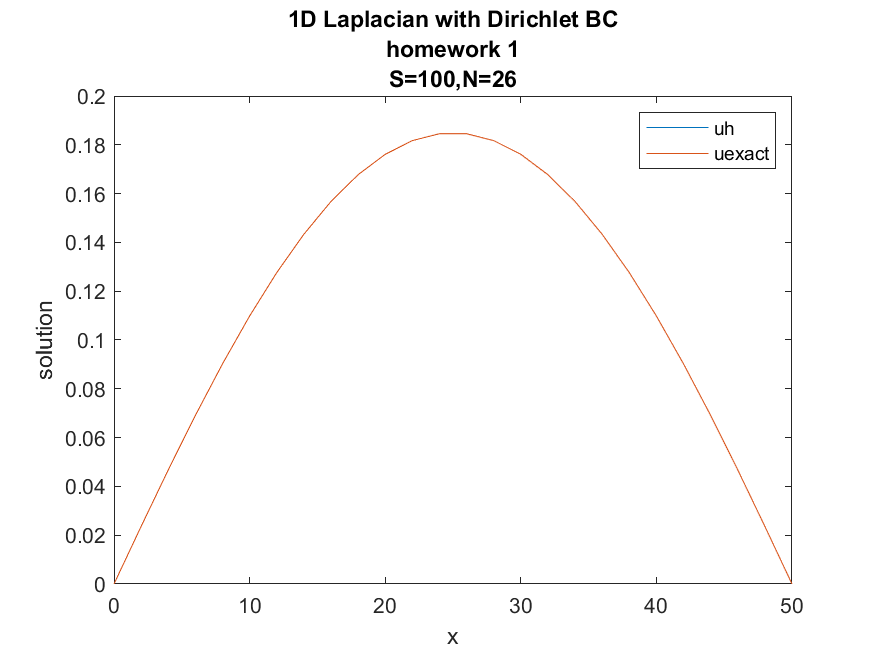
\includegraphics[scale=0.25]{hm1_S100_N26_sl}
		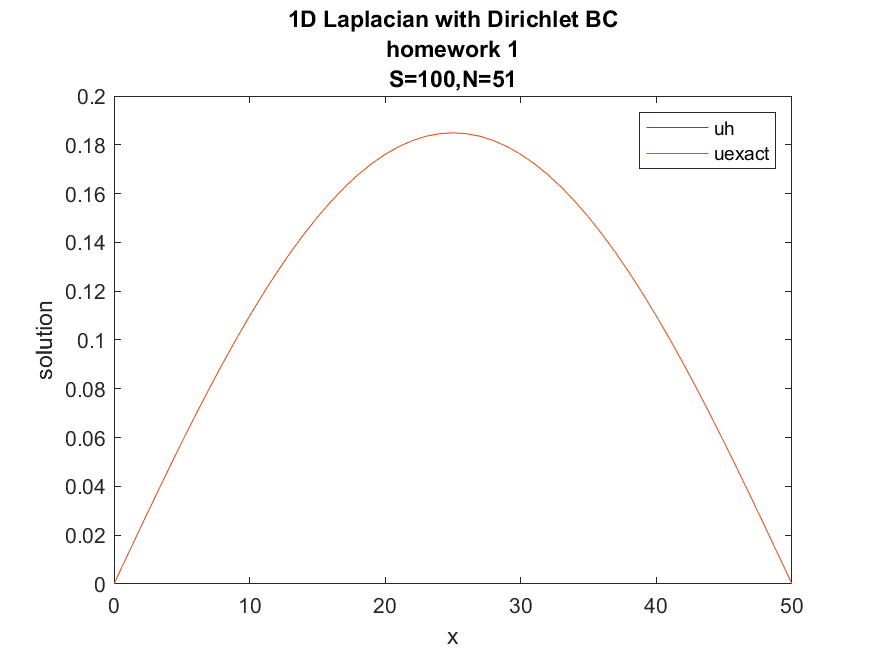
\includegraphics[scale=0.25]{hm1_S100_N51_sl}
		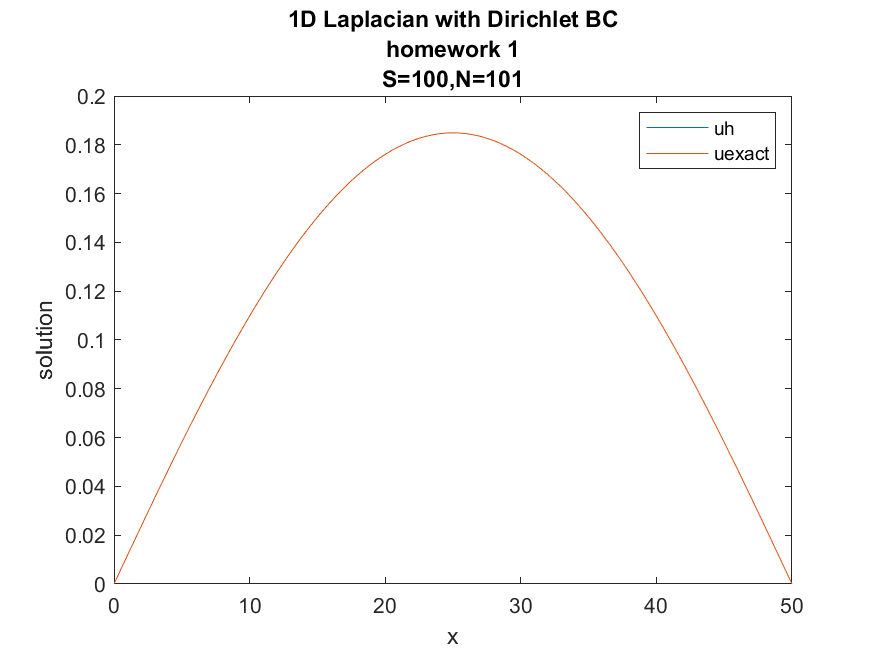
\includegraphics[scale=0.25]{hm1_S100_N101_sl}
		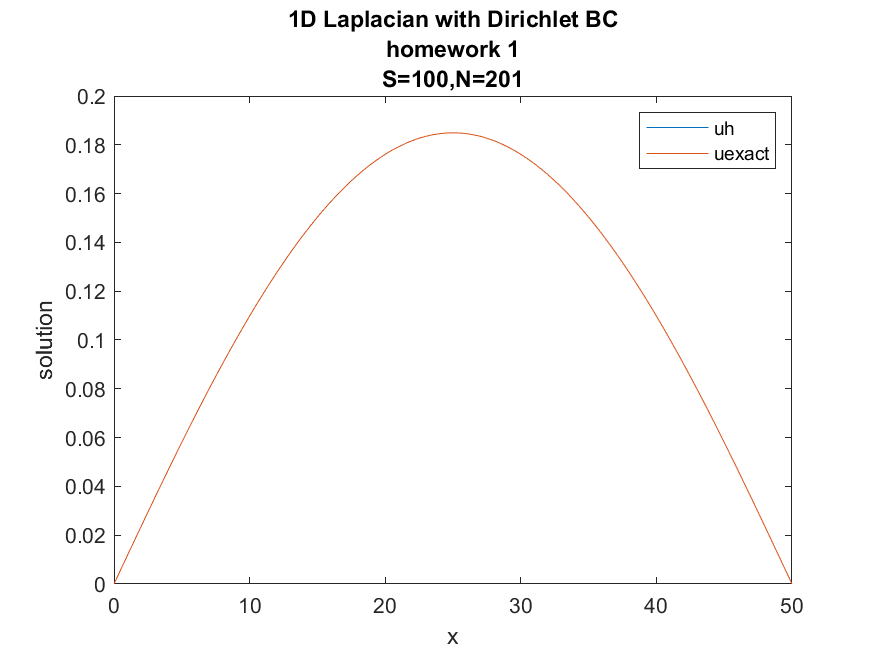
\includegraphics[scale=0.25]{hm1_S100_N201_sl}
		
		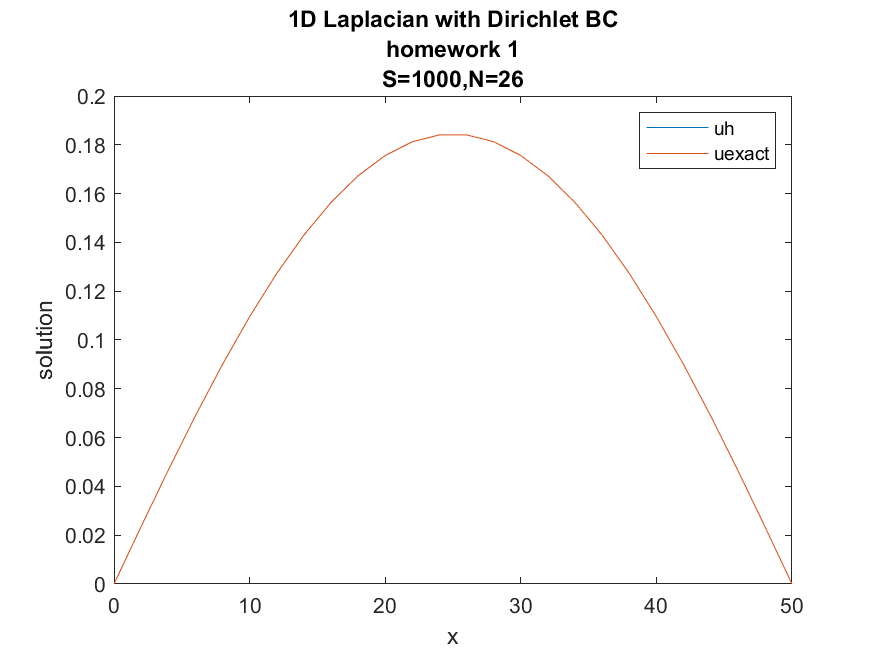
\includegraphics[scale=0.25]{hm1_S1000_N26_sl}
		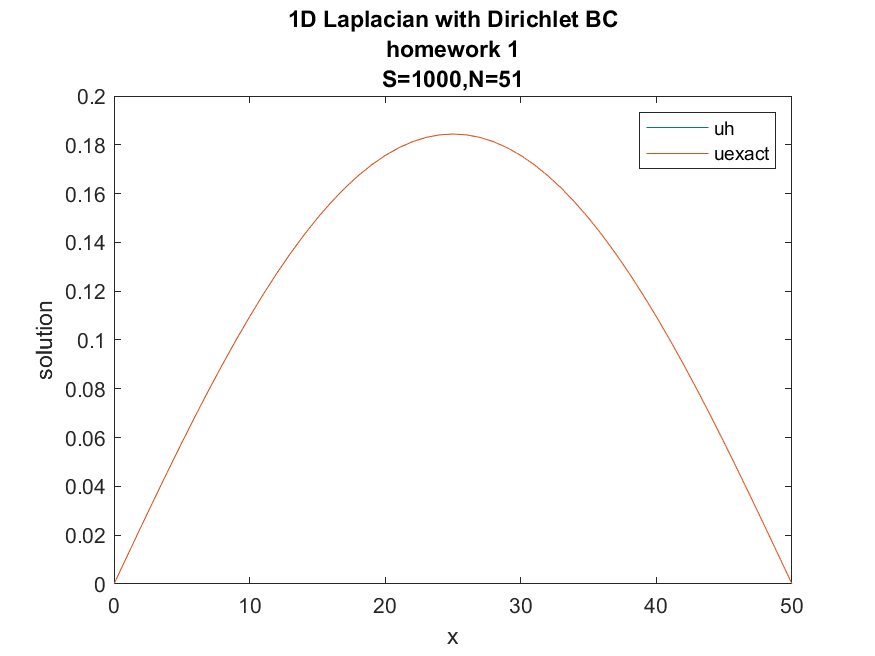
\includegraphics[scale=0.25]{hm1_S1000_N51_sl}
		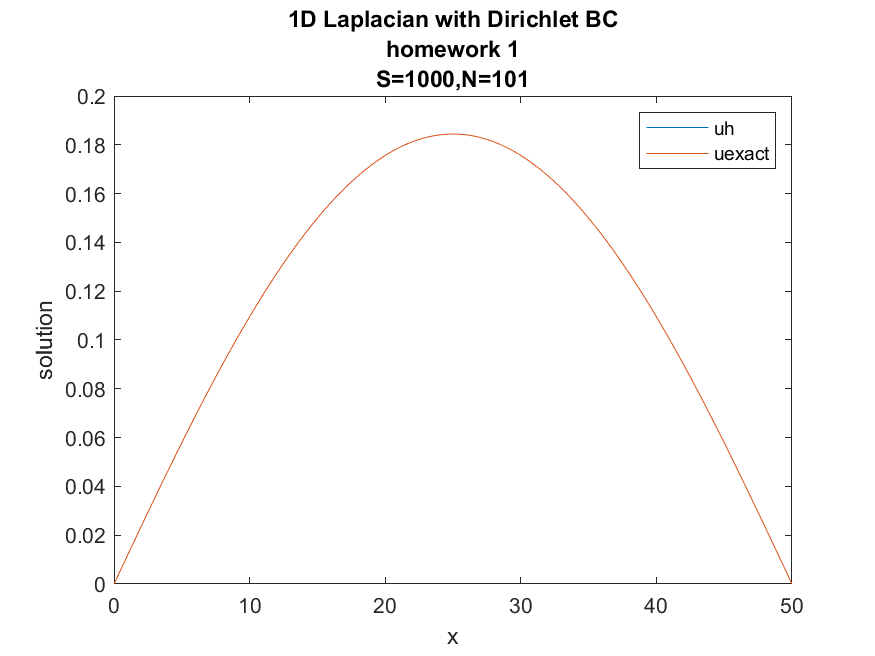
\includegraphics[scale=0.25]{hm1_S1000_N101_sl}
		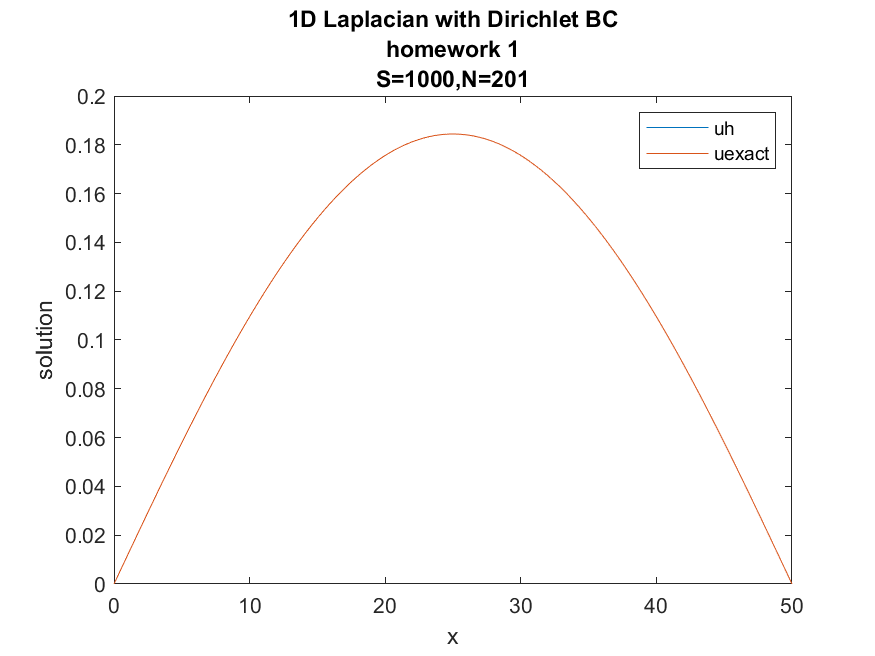
\includegraphics[scale=0.25]{hm1_S1000_N201_sl}
		
		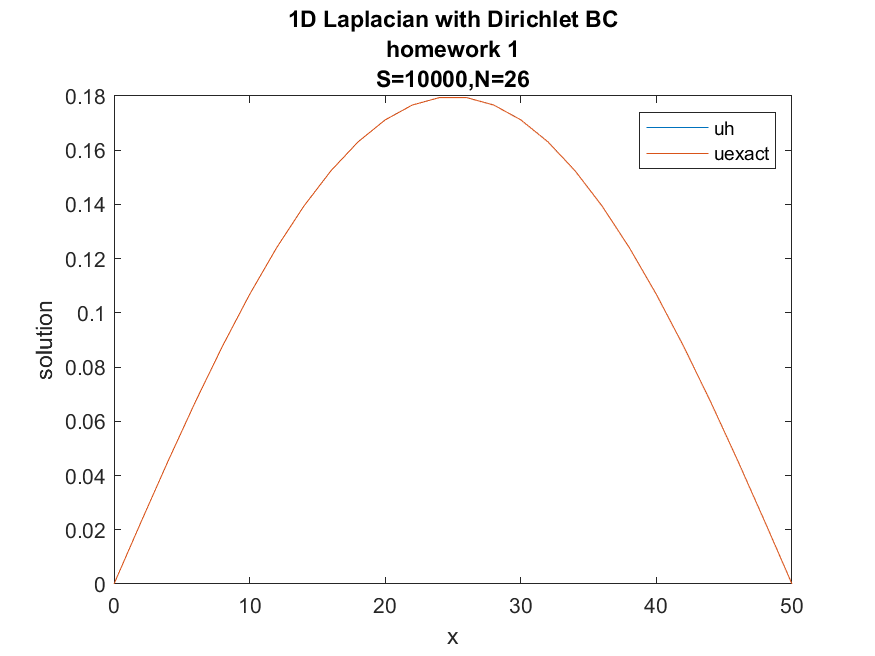
\includegraphics[scale=0.25]{hm1_S10000_N26_sl}
		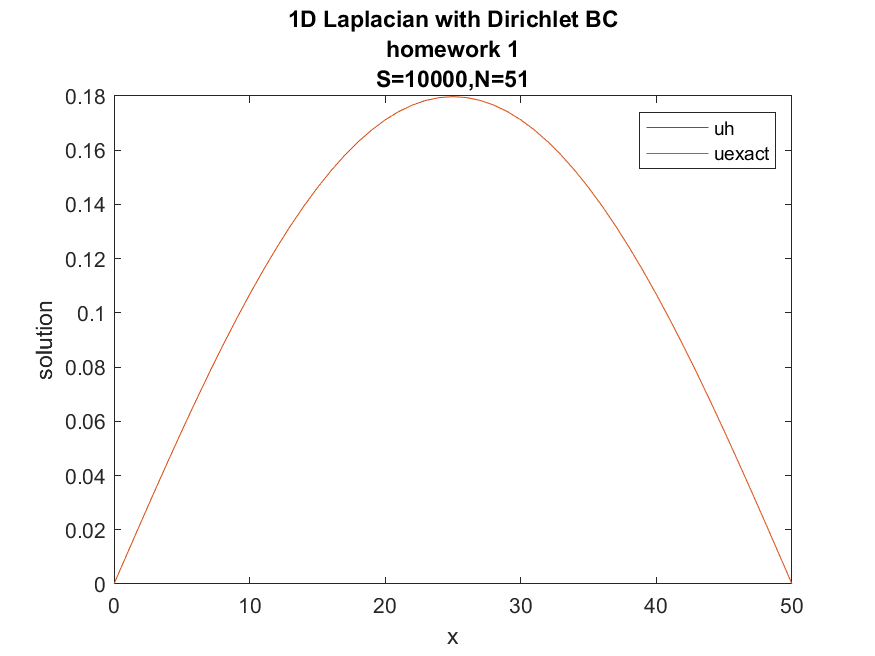
\includegraphics[scale=0.25]{hm1_S10000_N51_sl}
		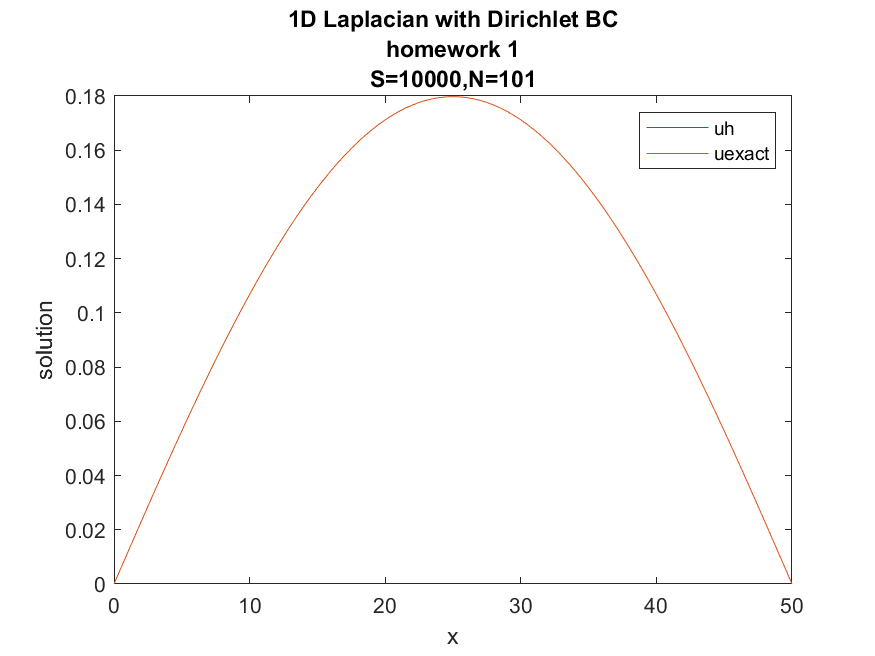
\includegraphics[scale=0.25]{hm1_S10000_N101_sl}
		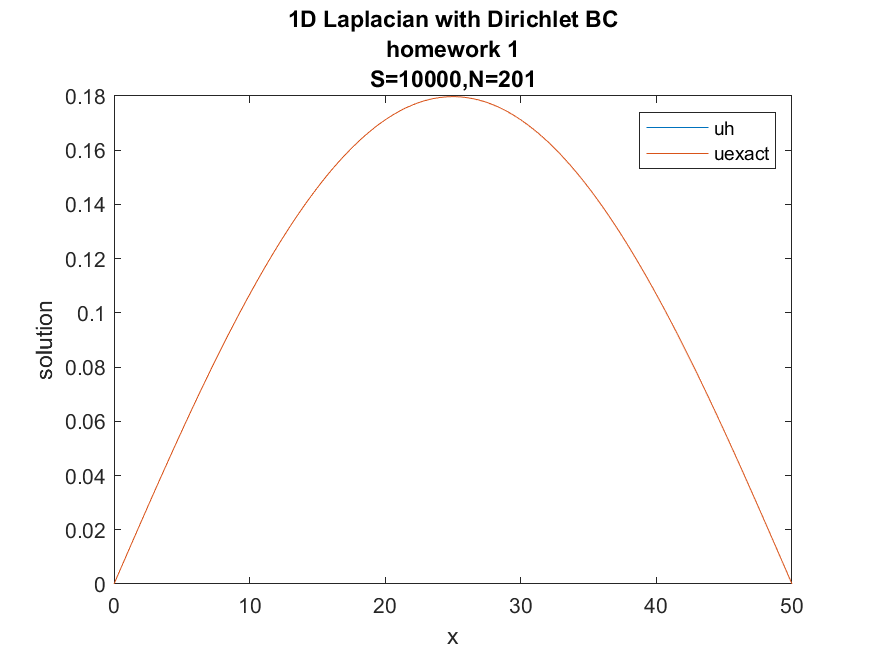
\includegraphics[scale=0.25]{hm1_S10000_N201_sl}		
	\end{center}
	The plot of error versus the mesh size is:\\
	\begin{center}
		\centering
		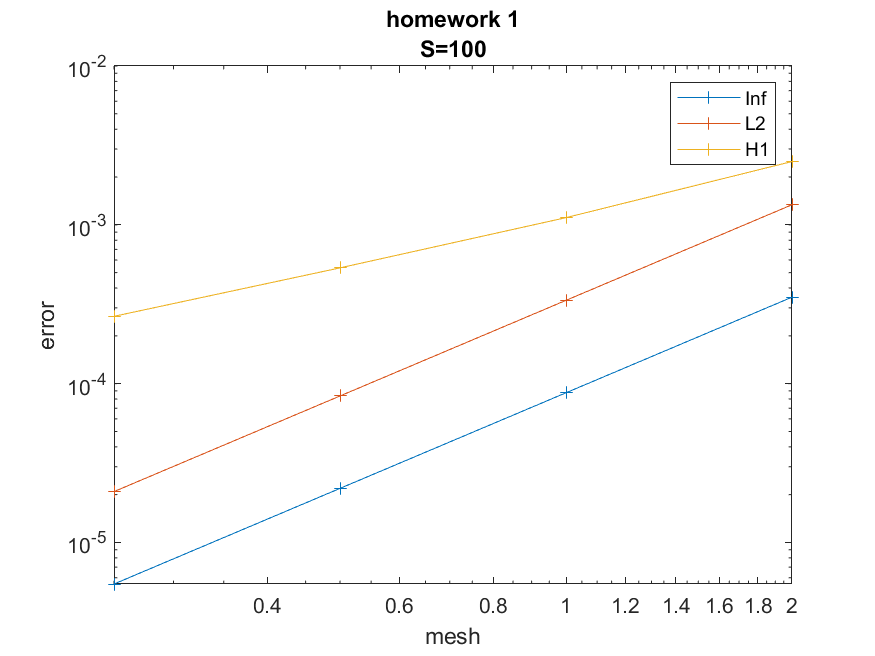
\includegraphics[scale=0.5]{hm1_S100}
		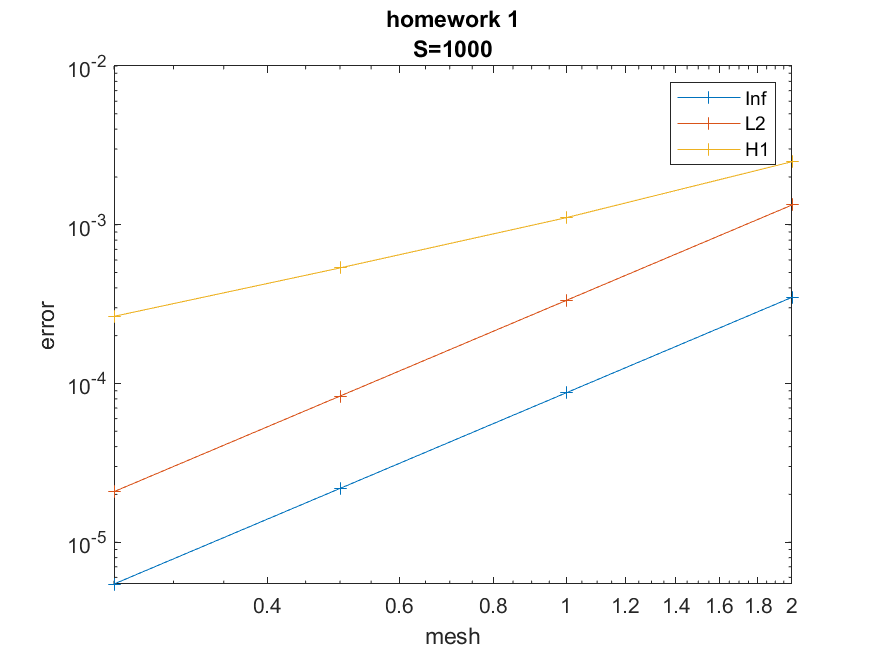
\includegraphics[scale=0.5]{hm1_S1000}
		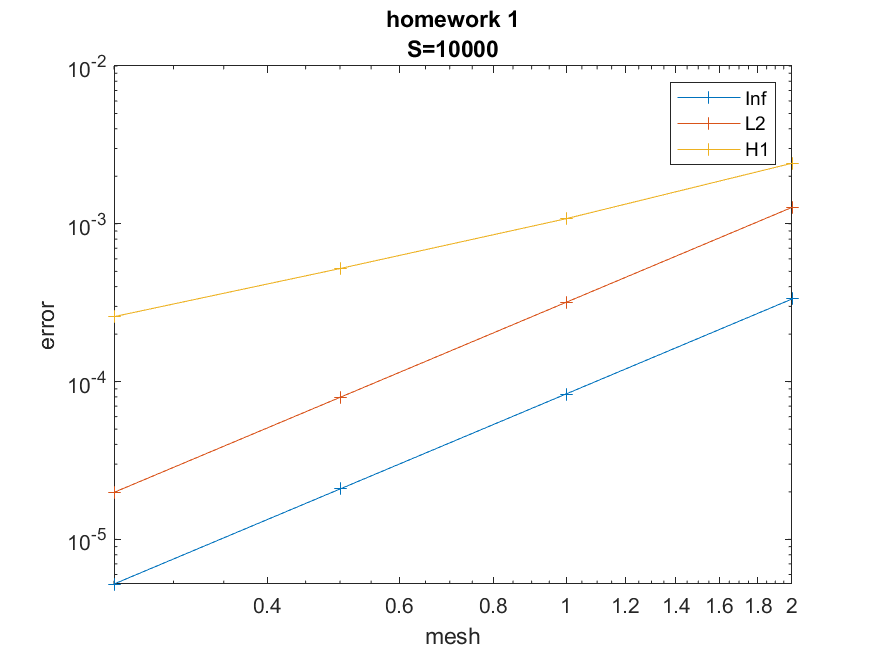
\includegraphics[scale=0.5]{hm1_S10000}	
	\end{center}
\end{figure}

\begin{table}
The error and convergence rate form is:\\
\begin{center}
\begin{tabular}{|c|c|c|c|c|c|c|c|c|} 
	\hline
S & num\_elements  & h & $\|u_h-u\|_{L^{2}}$ & $L^{2}$ rate & $\|u_h-u\|_{H^{1}}$ & $H^{1}$ rate & $\|u_h-u\|_{L^{\infty}}$ & $L^{\infty}$ rate  \\ \hline
   100 &  25   &   2  &  1.34e-03   &  0     &   2.50e-03 & 0 & 3.50e-04 & 0 \\
   100 &  50   &   1 &  3.35e-04   &  2     &   1.11e-03 & 1.17 & 8.76e-05 & 2 \\
   100 &  100   &   0.5  &  8.37e-05   &  2     &   5.36e-04 & 1.05 & 2.19e-05 & 2 \\
   100 & 200   &   0.25  &  2.09e-05   &  2     &   2.65e-04 & 1.01 & 5.48e-06 & 2 \\
   1000 &  25   &   2  &  1.33e-03   &  0     &   2.50e-03 & 0 & 3.49e-04 & 0 \\
   1000 &  50   &   1 &  3.33e-04   &  2     &   1.11e-03 & 1.17 & 8.72e-05 & 2 \\
   1000 &  100   &   0.5  &  8.33e-05  &  2     &   5.34e-04 & 1.05 & 2.18e-05 & 2 \\
   1000 & 200   &   0.25  &  2.08e-05  &  2     &   2.65e-04 & 1.01 & 5.45e-06 & 2 \\
   10000 &  25   &   2  &  1.27e-03   &  0     &   2.42e-03 & 0 & 3.34e-04 & 0 \\
   10000 &  50   &   1 &  3.18e-04   &  2     &   1.08e-03 & 1.17 & 8.35e-05 & 2 \\
   10000 &  100   &   0.5  &  7.95e-05   &  2     &   5.21e-04 & 1.05 & 2.09e-05 & 2 \\
   10000 & 200   &   0.25  &  1.99e-05   &  2     &   2.58e-04 & 1.01 & 5.22e-06 & 2 \\
	\hline
\end{tabular}
\end{center}
\end{table}

\newpage
\section{Problem 2}
There are too many results, we only give the results for case S=10000.\\ 
\begin{figure}
	The result plot is:\\
	\begin{center}
		\centering
		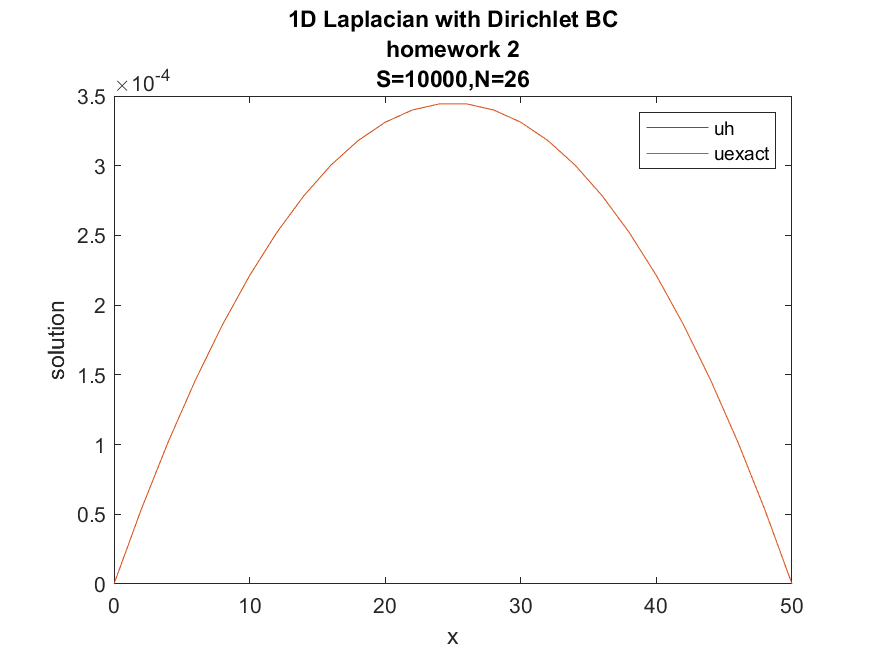
\includegraphics[scale=0.5]{hm2_S10000_N26_sl}
		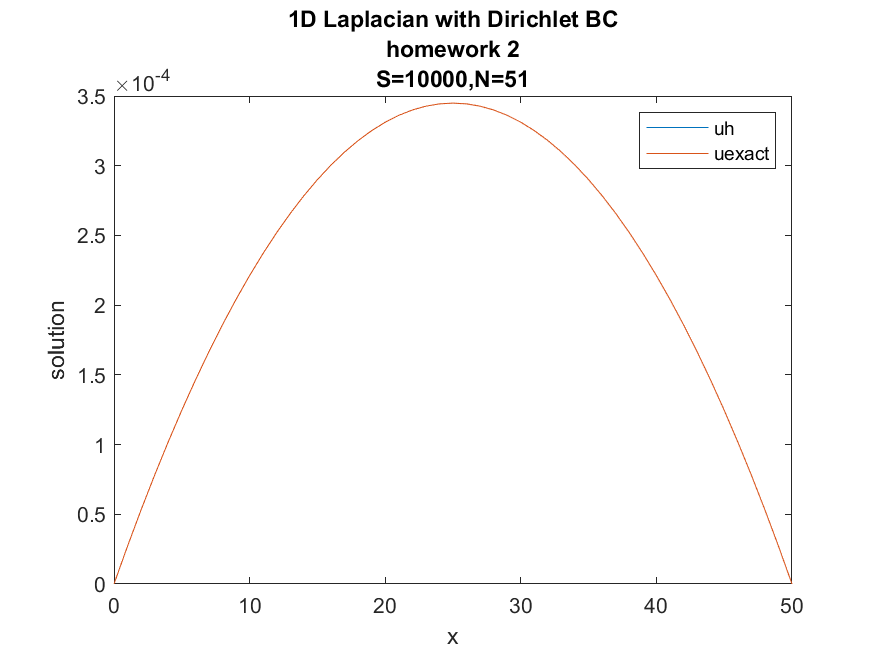
\includegraphics[scale=0.5]{hm2_S10000_N51_sl}
		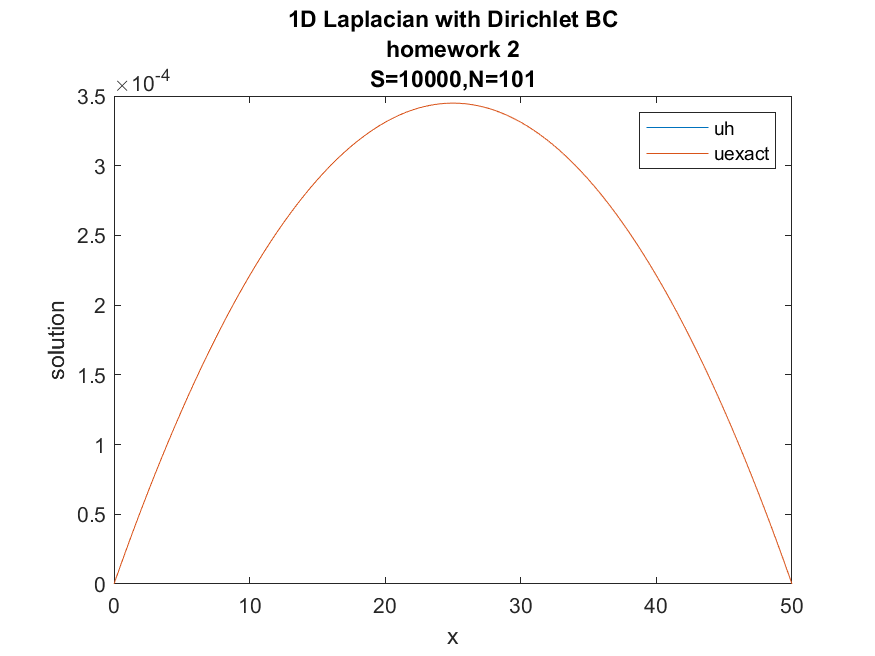
\includegraphics[scale=0.5]{hm2_S10000_N101_sl}
		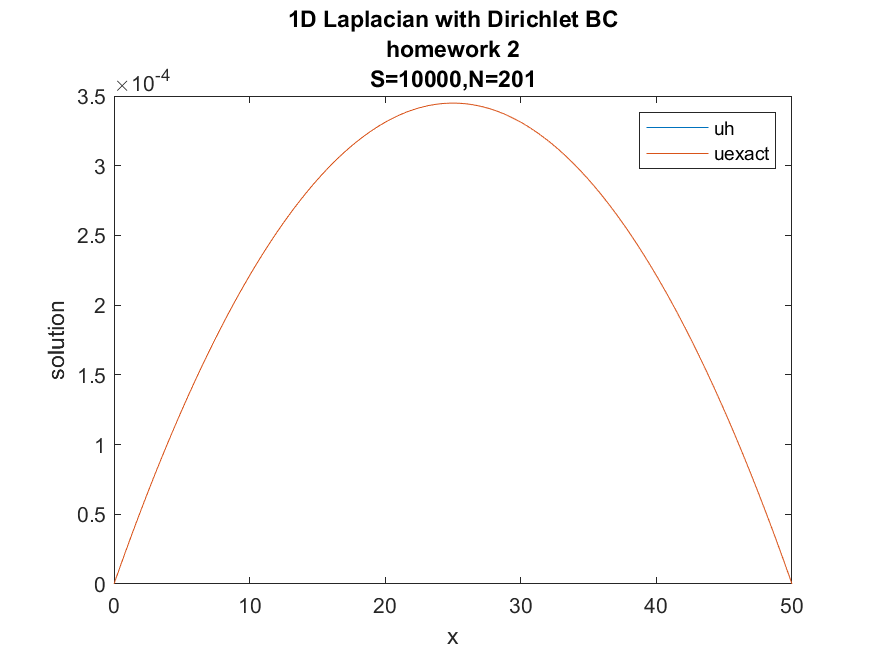
\includegraphics[scale=0.5]{hm2_S10000_N201_sl}		
	\end{center}

	The plot of error versus the mesh size is:\\
	\begin{center}
		\centering
		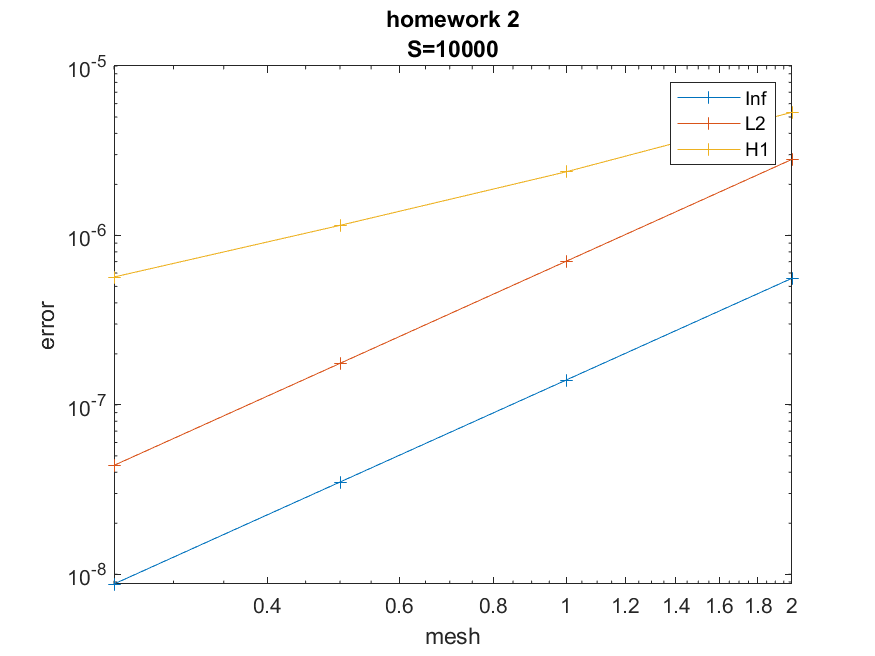
\includegraphics[scale=0.5]{hm2_S10000}	
	\end{center}
\end{figure}

\begin{table}
	The error and convergence rate form is:\\
	\begin{center}
		\begin{tabular}{|c|c|c|c|c|c|c|c|c|} 
			\hline
			S & num\_elements  & h & $\|u_h-u\|_{L^{2}}$ & $L^{2}$ rate & $\|u_h-u\|_{H^{1}}$ & $H^{1}$ rate & $\|u_h-u\|_{L^{\infty}}$ & $L^{\infty}$ rate  \\ \hline
			10000 &  25   &   2  &  2.81e-06   &  0     &   5.33e-06 & 0 & 5.59e-07 & 0 \\
			10000 &  50   &   1 &  7.03e-07   &  2     &   2.37e-06 & 1.17 & 1.40e-07 & 2 \\
			10000 &  100   &   0.5  &  1.76e-07   &  2     &  1.15e-06 & 1.05 & 3.50e-08 & 2 \\
			10000 & 200   &   0.25  &  4.39e-08   &  2     &   5.68e-07 & 1.01 & 8.76e-09 & 2 \\
			\hline
		\end{tabular}
	\end{center}
\end{table}




\section{Problem 3}
There are too many results, we only give the results for case S=10000.\\ 
\begin{figure}
	The result plot is:\\
	\begin{center}
		\centering
		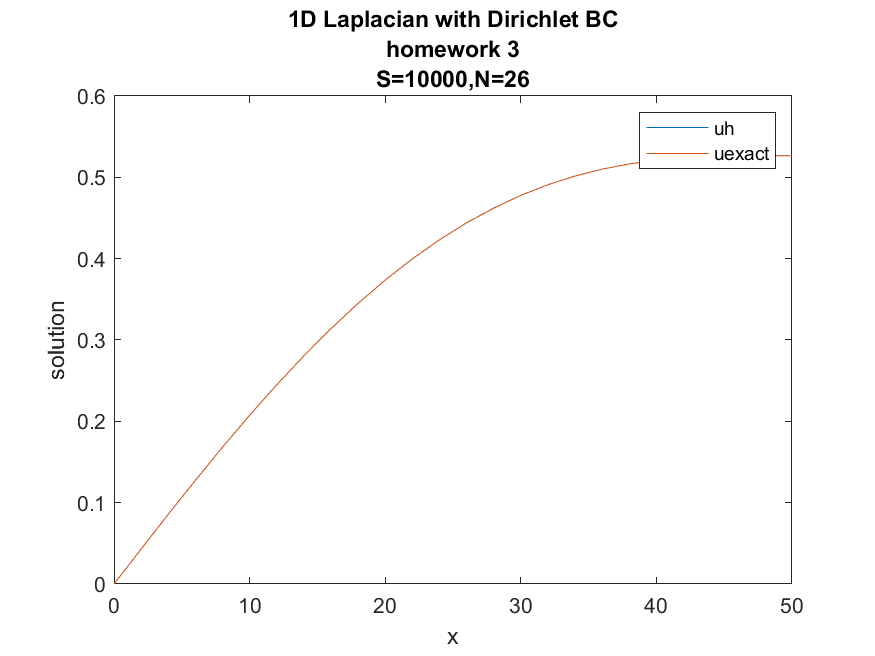
\includegraphics[scale=0.5]{hm3_S10000_N26_sl}
		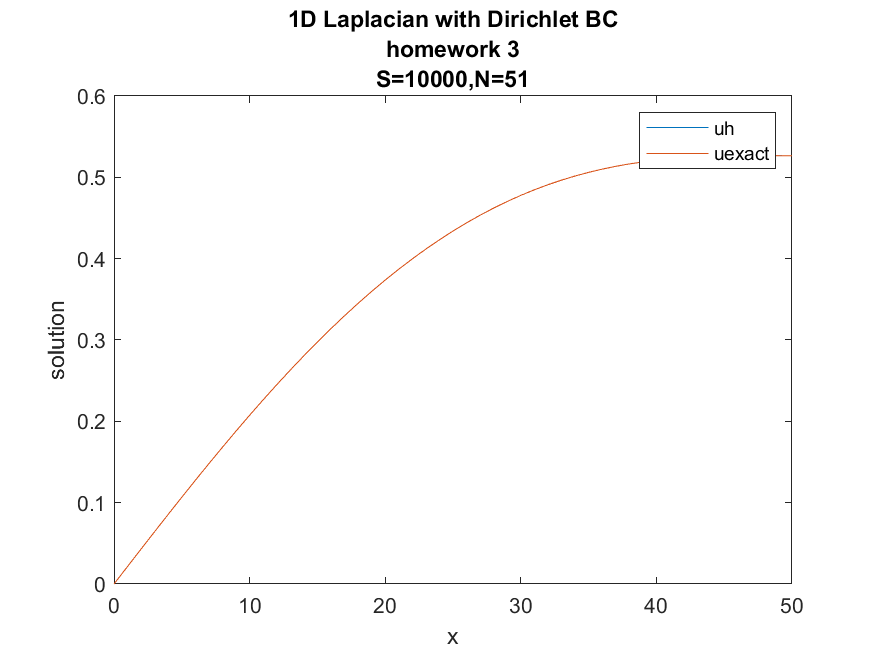
\includegraphics[scale=0.5]{hm3_S10000_N51_sl}
		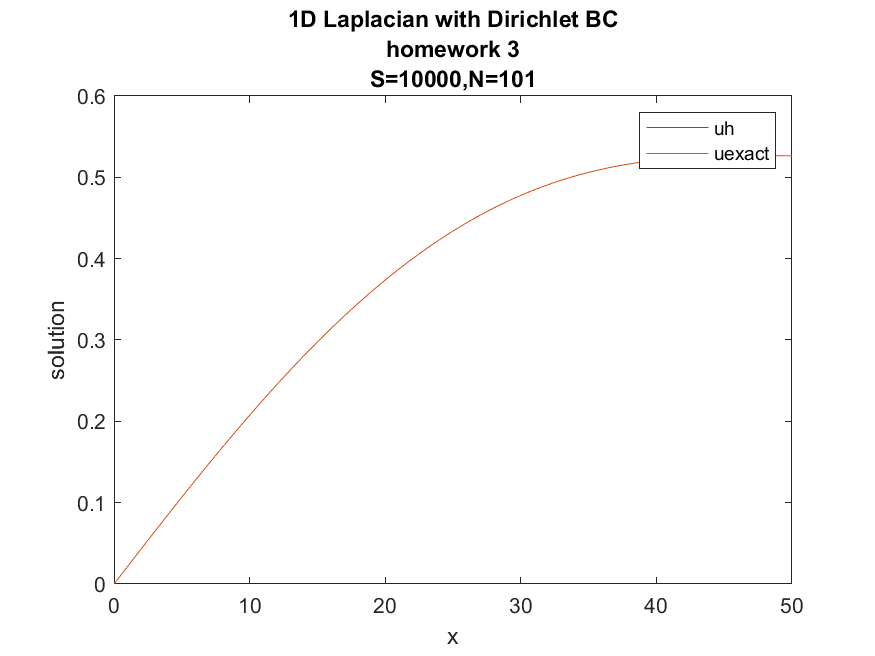
\includegraphics[scale=0.5]{hm3_S10000_N101_sl}
		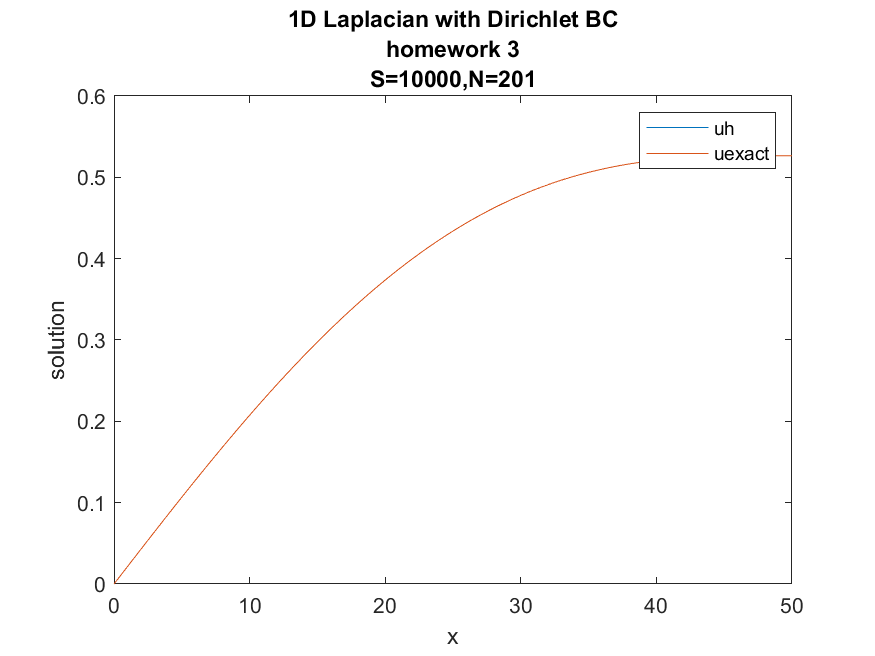
\includegraphics[scale=0.5]{hm3_S10000_N201_sl}		
	\end{center}
	The plot of error versus the mesh size is:\\
	\begin{center}
		\centering
		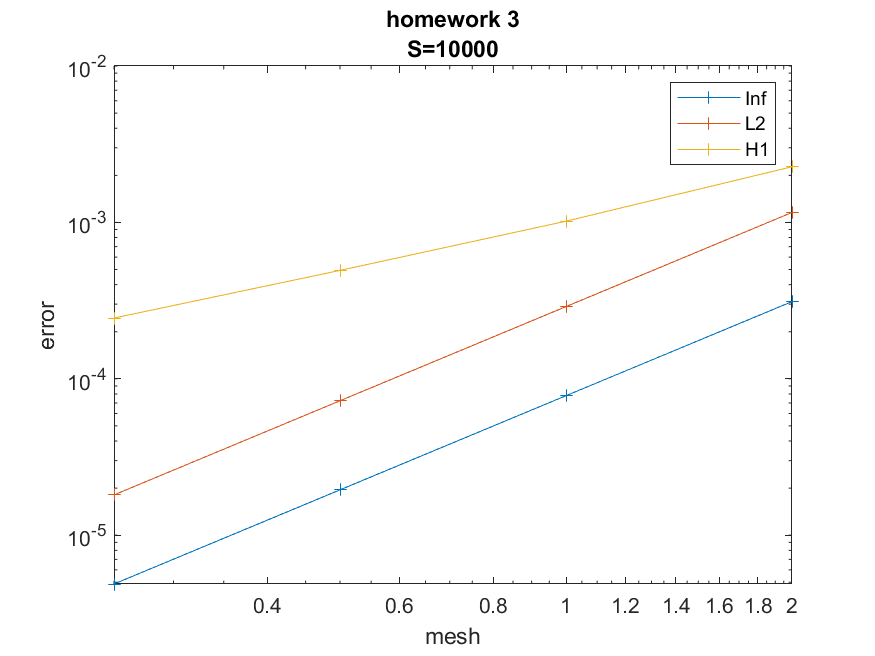
\includegraphics[scale=0.5]{hm3_S10000}	
	\end{center}
\end{figure}

\begin{table}
	The error and convergence rate form is:\\
	\begin{center}
		\begin{tabular}{|c|c|c|c|c|c|c|c|c|} 
			\hline
			S & num\_elements  & h & $\|u_h-u\|_{L^{2}}$ & $L^{2}$ rate & $\|u_h-u\|_{H^{1}}$ & $H^{1}$ rate & $\|u_h-u\|_{L^{\infty}}$ & $L^{\infty}$ rate  \\ \hline
			10000 &  25   &   2  &  1.16e-03   &  0     &   2.27e-03 & 0 & 3.12e-04 & 0 \\
			10000 &  50   &   1 &  2.90e-04   &  2     &   1.02e-03 & 1.16 & 7.80e-05 & 2 \\
			10000 &  100   &   0.5  &  7.24e-05   &  2     &  4.93e-04 & 1.05 & 1.95e-05 & 2 \\
			10000 & 200   &   0.25  &  1.81e-05   &  2     &   2.45e-04 & 1.01 & 4.87e-06 & 2 \\
			\hline
		\end{tabular}
	\end{center}
\end{table}


\section{Problem 4}
There are too many results, we only give the results for case S=10000.\\ 
\begin{figure}
	The result plot is:\\
	\begin{center}
		\centering
		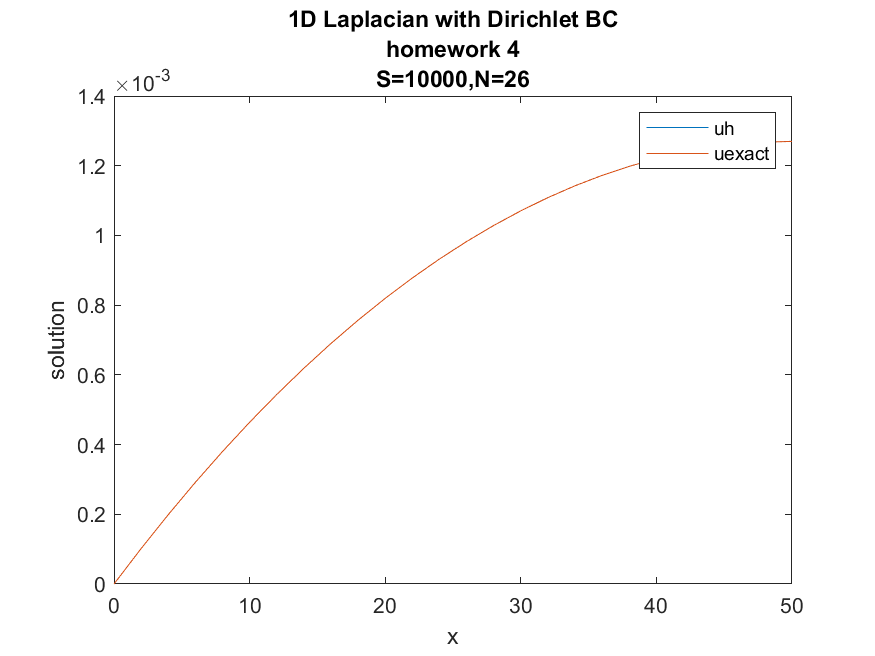
\includegraphics[scale=0.5]{hm4_S10000_N26_sl}
		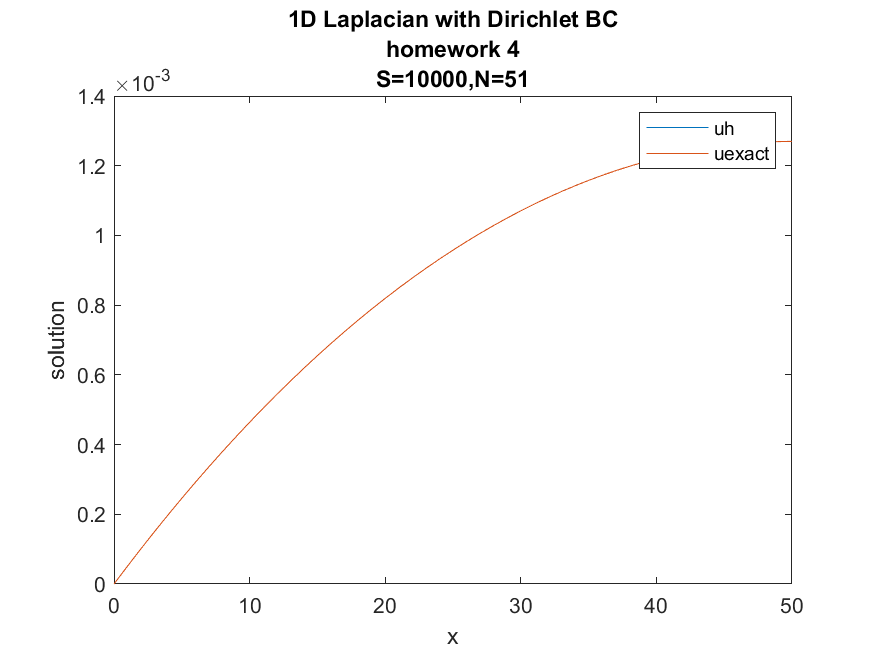
\includegraphics[scale=0.5]{hm4_S10000_N51_sl}
		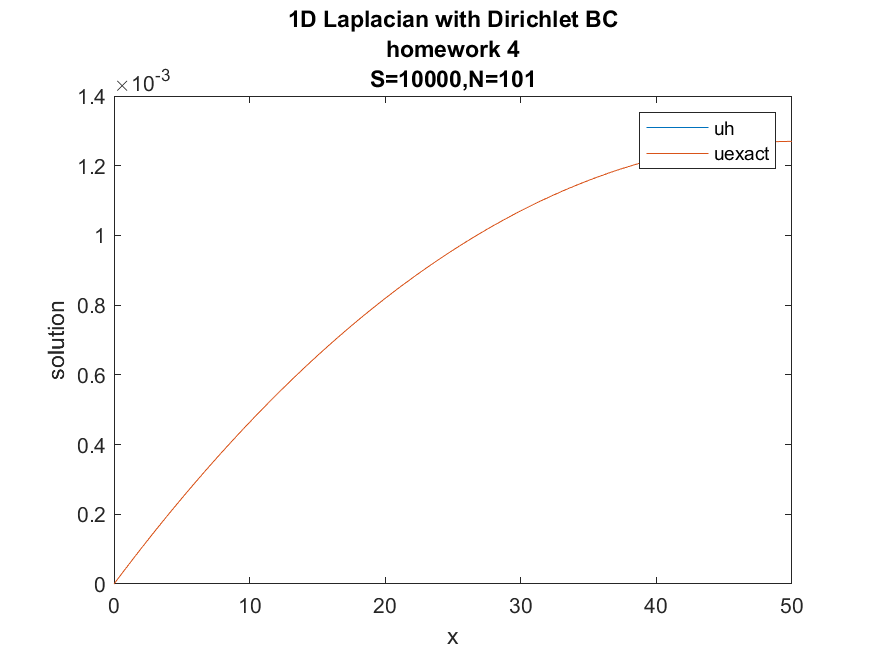
\includegraphics[scale=0.5]{hm4_S10000_N101_sl}
		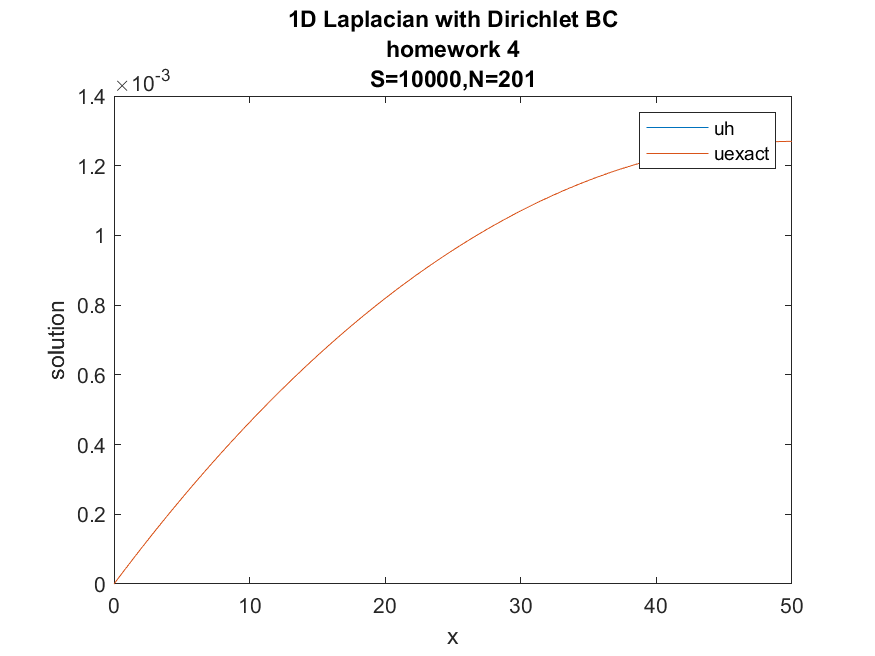
\includegraphics[scale=0.5]{hm4_S10000_N201_sl}		
	\end{center}
	The plot of error versus the mesh size is:\\
	\begin{center}
		\centering
		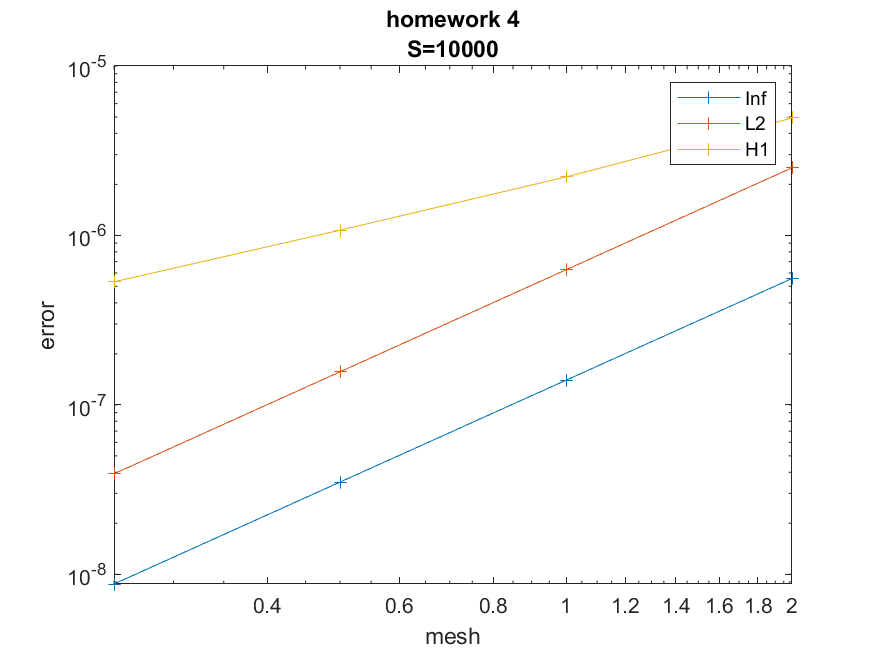
\includegraphics[scale=0.5]{hm4_S10000}	
	\end{center}
\end{figure}

\begin{table}
	The error and convergence rate form is:\\
	\begin{center}
		\begin{tabular}{|c|c|c|c|c|c|c|c|c|} 
			\hline
			S & num\_elements  & h & $\|u_h-u\|_{L^{2}}$ & $L^{2}$ rate & $\|u_h-u\|_{H^{1}}$ & $H^{1}$ rate & $\|u_h-u\|_{L^{\infty}}$ & $L^{\infty}$ rate  \\ \hline
			10000 &  25   &   2  &  2.51e-06   &  0     &   4.93e-06 & 0 & 5.57e-07 & 0 \\
			10000 &  50   &   1 &  6.27e-07   &  2     &   2.21e-06 & 1.16 & 1.40e-07 & 2 \\
			10000 &  100   &   0.5  &  1.57e-07   &  2     &   1.07e-06 & 1.04 & 3.50e-08, & 2 \\
			10000 & 200   &   0.25  &  3.92e-08	   &  2     &   5.32e-07 & 1.01 & 8.76e-09 & 2 \\
			\hline
		\end{tabular}
	\end{center}
\end{table}


\section{Summary}
From the plot and the table, we know that\\
(1)The smaller the mesh size is, the smaller the error is.\\
(2)The result of simulation is quite good, even for n=25.\\
(3)The shrink rate of error should be exponential level, since the error versus mesh size is almost linear and we use loglog function to plot it.\\
(4)The error in different norm has the same order of magnitude. For $L^{2}$ and $L^{\infty}$ norm, we expect to see order 2 convergence for small enough mesh size which is confirmed above by experiment. For $H^{1}$ norm, we expect to see order 1 convergence for small enough mesh size which is confirmed above by experiment.
\end{document}








